\documentclass[11pt,a4paper,uplatex,dvipdfmx]{ujarticle} 		% for uplatex
%\documentclass[11pt,a4j,dvipdfmx]{jarticle} 					% for platex
%=======================================
% form00_header.tex
%	General header for kakenhiLaTeX,  Moved over from form00_2010_header.tex.
%	2009-09-06 Taku Yamanaka (Osaka Univ.)
%==== General Version History ======================================
% 2006-05-30 Taku Yamanaka (Physics Dept., Osaka Univ.)
% 2006-06-02 V1.0
% 2006-06-14 V1.1 Use automatic calculation for cost tables.
% 2006-06-18 V1.2 Split user's contents and the format.
% 2006-06-20 V1.3 Reorganized user and format files
% 2006-06-25 V1.4 Readjusted all the table column widths with p{...}.
%				With \KLTabR and \KLTabRNum, now the items can be right-justified
%				in the cell defined by p{...}.
% 2006-06-26 V1.5 Use \newlength and \setlength, instead of \newcommand, to define positions.
% 2006-08-19 V1.6 Remade it for 2007 JFY version.
% 2006-09-05 V1.7 Added font declarations suggested by Hoshino@Meisei Univ.
% 2006-09-06 V1.8 Introduced usePDFform flag to switch the form file format.
% 2006-09-09 V1.9 Changed p.7, to allow different heights between years. (Thanks to Ytow.)
% 2006-09-11 V2.0 Added an option to show budget summary.
% 2006-09-13 V2.1 Added an option to show the group.
% 2006-09-14 V2.1.1 Cleaned up Kenkyush Chosho.
% 2006-09-21 V2.2 Generated under a new automatic development system.

% 2007-03-24 V3.0 Switched to a method using "picture" environment.

% 2007-08-14 V3.1 Switched to kakenhi3.sty.
% 2007-09-17 V3.2 Added \KLMaxYearCount
% 2008-03-08 V3.3 Remade it for 2009 JFY version\
% 2008-09-08 V3.4 Added \KLXf ... \KLXh.
% 2011-10-20 V5.0 Use kakenhi5.sty, to utilize array package in tabular environment.
% 2012-08-14 v5.1 Moved preamble and kakenhi5 into the current directory, instead of the parent directory.
% 2012-11-10 v6.0 Switched to kakenhi6.sty.
% 2015-08-26 v6.1 Added KLFirstPageIsLongPage flag.
% 2017-05-27 v7.0 Simplified for the new format.
%=======================================
% Dummy section and subsection commands.
% With these, some editors (such as TeXShop, etc.) can jump to the (sub)sections.
\newcommand{\dummy}{dummy}% 
\renewcommand{\section}[1]{\renewcommand{\dummy}{#1}}

\usepackage{calc}
\usepackage{geometry}                % See geometry.pdf to learn the layout options. There are lots.
\usepackage[dvipdfmx]{graphicx}
\usepackage{color}
\usepackage{ifthen}
\usepackage{udline}
\usepackage{array}
\usepackage{longtable}
\usepackage{fancyhdr}
 % pieces
%==================================================
% kakenhi7.sty
%==================================================
% v1
% Minimum amount of macros for writing Kakenhi forms.
%
% 2005-10-24 Taku Yamanaka, Physics Dept. Osaka Univ.
%		taku@hep.sci.osaka-u.ac.jp
% 		Macros such as XYBC, etc. were imported from Kakenhi Macro at
% 		http://www.yukawa.kyoto-u.ac.jp/contents/researcher/kakenhi.html .
% 2006-06-04 Taku
%		Added macros to draw boxes if \DrawBox is in the source.
%		This is useful when designing the LaTeX forms.
% 2006-06-14 Taku
%		Added LaTeX macros to add costs 
%		(\KLResetGrandSum, \KLCostItem, \KLSum, \KLGrandSum).
%		Added a macro \Number to supply commas every 3 digits (imported from kkh.mac).
% 2006-06-25 Taku
%		Added \KLTabC, \KLTabR, \KLTabRNum to specify alignments in tables.
%		Please note that \phantom{...} is required for the column, 
%		or otherwise somehow p{...mm} is ignored.
% 2006-08-13 Taku
%		Added \KLItemNumUnitCost . This requires calc.sty.
% 2006-09-06 Taku
%		Added KLGrandTotalValue to add ALL the costs.
%		Also added \KLPrintGrandTotal to print the total on the console.
% 2006-09-09 Taku
%		Added macros to handle "efforts".
% 2006-09-10 Taku
%		Added \KLnewcounter to make series of counters.
%		Modified \KLResetGrandSum and \KLSum to add the sum for 
%		each category and year.
% 2006-09-11 Taku
%		Added \NumC to display LaTeX counter with commas.
% 2006-09-12 Taku
%		Added simple macros to make group table.
% 2006-09-23 Taku
%		Added the 'Fair License' notification.
% 2006-10-22 Taku
%		Initialize KLNumPeople to -1, so that the first header row will not be included in the count.
%====================================================
% v2
% 2007-03-24 Taku
%		Instead of using Kakenhi Macros to position items, 
%		switched to a new method using
%		"picture" environment.  The origin of the coordinate is set to 
%		the lower left corner of the paper.  The positions are given in "points", 
%		as can be read by gv. These methods were suggested by 
%		Tsutomu Sakurai at Saitama Univ..
% 2007-03-30 Taku
%		The sum of each category and year is made using 
%		macros \KLItemCost, etc., instead of \KLSum.  This is a step toward
%		automatically aligning category sums in the same year, in some forms.
% 2007-04-02 Taku
%		Added \KLBudgetMiniTabular, \KLMiniSum, etc. to handle
%		budget tables with multiple category columns.
% 2007-05-04 Taku
%		Added \multicolumnDottedLine .
%==================================================
% v3 
% 2007-08-14 Taku
%		Simplified page handling, by introducing \KLBeginSinglePage,
%		\KLPageRange, etc..
% 2007-09-01 Taku
%		Added a new command, \KLItemNumUnitCostLocation , 
%		and \KLAddCost to clean things up.
% 2007-09-06 Taku
%		Set \KLEven/OddLeft/RightEdge parameters in \KLWaterMark.
%		Without it, if \KLLeftEdge or \KLRightEdge is used inside watermark,
%		it generated a very obscure error message, which was hard to track down.
% 2007-09-09 Taku
%		Removed clearring \thiswatermark in \KLClearWaterMarks.
% 2007-09-12 Taku
%		Added \KLPriorityItemNumUnitCostTwo for Tokusui.
% 2007-09-14 Taku
%		Added \KLItemNumUnitCostTwo for tokutei_koubo.
% 2007-09-17 Taku
%		In \KLAddCost, costs are added only if it is within the defined year range.
% 2008-09-02 Taku
%		  Added \KLMonthPriorityItemNumUnitCostTwo for tokutei_keizoku.
% 2008-09-07 Taku
%		   Use \KLJFY to print year in budget tables.
% 2008-10-21 Taku
%			Added KLItemNumUnitCostInParen for shorei.
% 2009-09-03 Taku
%			Added \dottedLine .
%==================================================
% v4
% 2009-09-06 Taku
%			Added macros for partial typesetting.
% 2009-09-12 Taku
%			Added macros for showing coordinates and edges.
% 2009-09-13 Taku
%			Added macros to show boxes and minipage frames and their corner coordinates.
% 2010-03-04 Taku
%			Moved macros for calculating lengths and positions from form07_header.tex to here.
% 2010-04-11 Taku
%			Added \KLItemCostOne for jisedai, and necessary flags to print budget sums before 
%			the detailed budget table.
%==================================================
% v5
% 2011-10-20 Taku
%			By using array package within tabular environment, the following macros were simplified:
%			\KLTabC, \KLTabR, \KLBudgetMiniTabular, 
%			New Macros:
%			\KLCC, \KLCR
% 2011-10-24 Taku
%			Removed using \KLTabR from most of the budget tables.
% 2011-10-26 Taku
%			Added KLMyBudget.
%			Modified KLYearItemNumUnitCostTwo to just put the JFY if the second item is blank.  (For Kiban S)
% 2012-03-10 Taku
%			Changed the tabcolsep for \KLMyBudget to 0pt.
% 2012-08-14 Taku
%			Moved xxx_forms_pdf and _eps directories to under mother.
% 2012-09-09	Taku
%			Added \KLbibitem(B) and \KLcite(B).
% 2012-09-16	Taku
%			Added \KLOtherApplication, \KLOtherApplicationReasons, and \KLOtherFundReasons
%			for tokusui (and maybe for others in the future).
%==================================================
% v6
% 2012-11-10	Taku
% 			Modified \KLOtherApplicationReasons and \KLOtherFundReasons to make the tables compact.
%			These were in hook3.tex for the 2013 version.
%			Added \KLOtherApplicationDiff for many shumokus.
%			Removed \KLbibitemB and \KLciteB.
%			Changed \KLbibitem to use a dedicated column for numbering.
% 2012-11-11	Taku
%			Added \KLItemSetCostLocationInfo and \KLItemCostInfo.
% 2013-09-19	Taku
%			Added \KLOtherPD and \KLOtherPDShort to enter JSPS PD for other funds.
% 2013-10-02	Taku
%			Changed \KLbibItem, not to use a dedicated column for numbering, 
%			because otherwise the label defined in \label{...} cannot be used in @currentlabel.
% 2014-09-22	Taku
%			Added \KLCL for filling narrow tabular cells in English.  
%			(Suggested by Frank Bennett.)
% 2014-11-08	Taku
%			Added an instruction in \KLCheckPageLimit.
% 2015-08-23	Taku
%			Added NumCk to show numbers divided by 1000 (truncated).
% 2015-08-24	Taku
%			Introduced \KLLongPage and \KLSimpleLongPage to offer floating environment in 
%			single-page-frames.
%=====================================================
% v7
%	Frames are gone!  Simplify kakenhiLaTeX to benefit from 
%	the new style.
% 2017-05-03	Taku
%			Added \KLAnotherFund .
% 2017-05-27	Taku
%			Made \KLBeginSubject and \KLEndSubject to handle new 
%			mother file style.
% 2017-08-17 Taku
%	Added \KLItemCostNoYear and \KLEndBudgetNoYear for kokusai_kyoudou.
% 2017-08-19	Taku
%			Updated \KLBeginSubject and \KLEndSubject to handle 
%			various headers.
% 2017-08-20	Taku
%			\KLBeginSubject calls \KLFirstPageStyle and \KLDefaultPageStyle
%			which should be defined for each shumoku (or JSPS/MEXT).
%			This is to pass the subject name etc. to the header.
% 2017-08-27	Taku
%			Set section number in \KLBeginSubject.
% 2017-08-29	Taku
%			Moved over KLShumokuFirstPageStyle and KLShumokuDefaultPageStyle.
%			Added jsps-abs-p1-header, jps-abs-subject-header, and 
%			jsps-abs-default-header as arguments to \KLShumoku***Header.
% 2017-09-02	Taku
%			Added \KLBeginSubjectWithHeaderCommands for more flexible header style.
% 2017-09-03	Taku
%			Added \vspace*{-4mm} after \includegraphics in \KLBeginSubject*.
% 2017-09-05	Taku
%			Removed now-the-old commands.
% 2020-01-02	Taku
%			Added more numbers to \KLJint for gakuhen_a.
% 2020-01-15	Taku
%			Changed the horizontal position (none --> -3mm) 
%			and the width of the top boxes for headers (\linewidth --> 1.02\linewidth)
%			to reproduce the original boxes.  
%			This became necessary because the margins were set correctly in form02_header.tex.
% 2021-01-29	Taku
%			Set section counter and reset subsection counter only if the section # is given for
%			\KLBeginSubject and \KLBeginSubjectWithHeaderCommands .
%=====================================================

%=====================================================
% Macro to supply commas every 3 digits (up to 9 digits)
%	Imported from kkh.mac for Kakenhi Macro.
%=====================================================
%
\newif\ifNumWithCommas \NumWithCommastrue
\def\NumWithCommas{\NumWithCommastrue}
\def\NumWithoutCommas{\NumWithCommasfalse}
\newcount\Numa
\newcount\Numb
\def\Numempty{}%output blank if "-0" is given
\def\Number#1{\edef\Numpar{#1}\ifx\Numempty\Numpar\else%
\ifNumWithCommas\Numa=#1\relax
\ifnum\Numa>999999\divide\Numa by 1000000
\number\Numa,%
\multiply\Numa by -1000000\advance\Numa by #1\relax
\Numb=\Numa\divide\Numa by 1000
\ifnum\Numa<100 \ifnum\Numa<10 0\fi0\fi\number\Numa,%
\multiply\Numa by -1000\advance\Numa by \Numb
\ifnum\Numa<100 \ifnum\Numa<10 0\fi0\fi\number\Numa%
\else\ifnum\Numa>999\divide\Numa by 1000
\number\Numa,%
\multiply\Numa by -1000\advance\Numa by #1\relax
\ifnum\Numa<100 \ifnum\Numa<10 0\fi0\fi\number\Numa%
\else\number\Numa\fi\fi\else\number#1\fi\fi}

%======================================================
% Macro to display LaTeX counter with commas every 3 digits.
%======================================================
\newcommand{\NumC}[1]{\Number{\value{#1}}}

\newcounter{kyen}
\newcommand{\NumCk}[1]{%
	\setcounter{kyen}{\arabic{#1}/1000}
	\Number{\value{kyen}}
}

%======================================================
% Macros to align (right-justify, center) elements within a tabular cell
% whose width is defined by p{...}.
% 2006-06-25 Taku
% 	These are necessary, because the cell width should be given explicitly
% 	by p{...mm} to match the given table in a tabular environment.  
% 	One could allocate a width with \phantom{...},
% 	but it is a little tricky, since it depends on the font size.
%======================================================

%---------------------------------------------------------------------
% Center text within a tabular cell allocated by p{...}
%\newcommand{\KLTabC}[1]{\multicolumn{1}{c}{#1}}
\newcommand{\KLTabC}[1]{\centering\arraybackslash#1}
% This new method does not require a dummy table row to put them in correct columns.
%
% This should be used in tabular definition, as:
%	\begin{tabular}[t]{>{\KLCC}p{30pt}p{50pt}}
\newcommand{\KLCC}{\centering\arraybackslash}

%---------------------------------------------------------------------
% Right justify text within a tabular cell allocated  by p{...}
%\newcommand{\KLTabR}[1]{\multicolumn{1}{r@{\ }}{#1}}
\newcommand{\KLTabR}[1]{\raggedleft\arraybackslash#1}

% This should be used in tabular definition, as:
%	\begin{tabular}[t]{>{\KLCR}p{30pt}p{50pt}}
\newcommand{\KLCR}{\raggedleft\arraybackslash}%

%---------------------------------------------------------------------
% Right justify number (with comma every 3 digits) 
% within a tabular cell allocated by p{...}
\newcommand{\KLTabRNum}[1]{\KLTabR{\Number{#1}}}

%---------------------------------------------------------------------
% Left justify text within a tabular cell allocated by p{...}
% This should be used in tabular definition, as:
%	\begin{tabular}[t]{>{\KLCL}p{30pt}p{50pt}}
\newcommand{\KLCL}{\raggedright\arraybackslash}%

%=================================================
%  counter tools
%=================================================
\newcounter{KLtmp}

%------------------------------------------------------------------------------
% Makes a set of counters, with prefix #1, followed by 
% suffix ranging from 0 to #2 - 1.
% For example, \KLnewcounter{mine}{3} makes counters
% mine0, mine1, and mine2 .
%-------------------------------------------------------------------------------
\newcommand{\KLnewcounter}[2]{
	\setcounter{KLtmp}{0}
	
	\whiledo{\value{KLtmp} < #2}{
		\newcounter{#1\arabic{KLtmp}}
		\stepcounter{KLtmp}
	}
}

%------------------------------------------------------------------------------
% Dumps the contents of the counters.
%------------------------------------------------------------------------------
\newcommand{\KLdumpcounter}[2]{
	\setcounter{KLtmp}{0}
	
	\whiledo{\value{KLtmp} < #2}{
		#1\arabic{KLtmp} : \arabic{#1\arabic{KLtmp}}\\
		\stepcounter{KLtmp}
	}
}

%=======================================================
% LaTeX macros to add costs.
%	2006-06-14 Taku Yamanaka
%=======================================================
\newcounter{KLCost}				% to calculate cost = #units x unit cost
\newcounter{KLGrandTotalValue}		% for the grand total of all the categories in all years
\setcounter{KLGrandTotalValue}{0}

\newcommand{\KLCostCategory}{KLequipments}
\newcounter{KLYearCount}
\newcounter{KLPrintYear}

% Make counters for annual sums for each category-----------------------
\newcommand{\KLMaxYear}{8}
\KLnewcounter{KLequipments}{\KLMaxYear}
\KLnewcounter{KLexpendables}{\KLMaxYear}
\KLnewcounter{KLdomestic}{\KLMaxYear}
\KLnewcounter{KLforeign}{\KLMaxYear}
\KLnewcounter{KLtravel}{\KLMaxYear}
\KLnewcounter{KLgratitude}{\KLMaxYear}
\KLnewcounter{KLmisc}{\KLMaxYear}
\KLnewcounter{KLAnnualSum}{\KLMaxYear}

%------------------------------------------------
% Add up the given cost to category-year sum, category sum, year-sum, and total.
% 2007-09-01 Taku
% 2007-09-17 Taku: Add costs only if it is within the defined year range.
%------------------------------------------------
\newcommand{\KLAddCost}[1]{%
	\ifthenelse{\value{KLYearCount} > \value{KLMaxYearCount}}{%
		%pass
	}{%
		\addtocounter{\KLCostCategory0}{#1}%
		\addtocounter{\KLCostCategory\arabic{KLYearCount}}{#1}%
		\addtocounter{KLAnnualSum\arabic{KLYearCount}}{#1}%
		\addtocounter{KLAnnualSum0}{#1}%
		\ifthenelse{\equal{\KLCostCategory}{KLdomestic}}{%
			\addtocounter{KLtravel0}{#1}%
			\addtocounter{KLtravel\arabic{KLYearCount}}{#1}%
		}{}%
		\ifthenelse{\equal{\KLCostCategory}{KLforeign}}{%
			\addtocounter{KLtravel0}{#1}%
			\addtocounter{KLtravel\arabic{KLYearCount}}{#1}%
		}{}%
	}%
}


\newcommand{\KLClearWaterMarks}{%
	%--empty watermarks
	\watermark{}
%	\thiswatermark{}
	\rightwatermark{}
	\leftwatermark{}
}

\newcommand{\KLInput}[1]{%	The macros defined inside the file are only valid within the file.
	\begingroup
	\input{#1}
	\endgroup
}

%================================
% For 2017 new style without frames
%================================
\newcommand{\KLShumokuFirstPageStyle}[5]{%
%	Defines the header for the first page.
%	Called from \KLBeginSubject.
%--------------------------------
%	#1: page style name
%	#2: 様式
%	#3: 研究種目名
%	#4: 項目名
%	#5: sectionNo
%--------------------------------
	\ifthenelse{\equal{#1}{jsps-p1-header}}{%
		\JSPSVeryFirstPageStyle{#1}{#2}{#3}{#4}{#5}
	}{%
		\ifthenelse{\equal{#1}{jsps-abs-p1-header}}{%
			\JSPSVeryFirstPageStyle{#1}{#2}{#3 概要}{#4}{#5}
		}{%
            		\ifthenelse{\equal{#1}{jsps-subject-header}}{%
            			\JSPSFirstSubjectPageStyle{#1}{#2}{#3}{#4}{#5}
            		}{%
				\ifthenelse{\equal{#1}{jsps-abs-subject-header}}{%
            				\JSPSFirstSubjectPageStyle{#1}{#2}{#3 概要}{#4}{#5}
				}{%
                    			\thispagestyle{#1}
				}
            		}
		}
	}
}

\newcommand{\KLShumokuDefaultPageStyle}[5]{%
%	Defines the default header.
%	Called from \KLBeginSubject.
%--------------------------------
%	#1: page style name
%	#2: 様式
%	#3: 研究種目名
%	#4: 項目名
%	#5: sectionNo
%--------------------------------
	\ifthenelse{\equal{#1}{jsps-default-header}}{%
		\JSPSDefaultPageStyle{#1}{#2}{#3}{#4}{#5}
	}{%
		\ifthenelse{\equal{#1}{jsps-abs-default-header}}{%
			\JSPSDefaultPageStyle{#1}{#2}{#3 概要}{#4}{#5}
		}{%
            		\pagestyle{#1}
		}
	}
}

\newcommand{\KLSubjectName}{}
\newcommand{\KLSubjectMaxPages}{}
\newcommand{\KLSubjectEndPage}{}
\newcounter{KLSubjectEndPage}
\setcounter{KLSubjectEndPage}{0}

\newcommand{\KLSubjectCheckNPages}{%
%	\arabic{page}, \arabic{KLSubjectEndPage}\\
	\ifthenelse{\value{page}>\value{KLSubjectEndPage}}{
		{\LARGE「\KLSubjectName」は \KLSubjectMaxPages\ ページ以内で書いてください。}
		\clearpage
	}{%
	}
}

\newcommand{\KLSubjectAdvancePages}{%
	\renewcommand{\KLSubjectEndPage}{\value{KLSubjectEndPage}}
	\ifthenelse{\value{page}<\KLSubjectEndPage}{%
		\phantom{x}\clearpage
	}{}
	% Advance page if necessary
	\ifthenelse{\value{page}<\KLSubjectEndPage}{%
		\phantom{x}\clearpage
	}{}
	% Advance page if necessary
	\ifthenelse{\value{page}<\KLSubjectEndPage}{%
		\phantom{x}\clearpage
	}{}
	% Advance page if necessary
	\ifthenelse{\value{page}<\KLSubjectEndPage}{%
		\phantom{x}\clearpage
	}{}
	% Advance page if necessary
	\ifthenelse{\value{page}<\KLSubjectEndPage}{%
		\phantom{x}\clearpage
	}{}
}	

\newcommand{\KLJInt}[1]{%
% Returns full-width numerical character.
	\ifthenelse{\equal{#1}{1}}{1}{%
	\ifthenelse{\equal{#1}{2}}{2}{%
	\ifthenelse{\equal{#1}{3}}{3}{%
	\ifthenelse{\equal{#1}{4}}{4}{%
	\ifthenelse{\equal{#1}{5}}{5}{%
	\ifthenelse{\equal{#1}{6}}{6}{%
	\ifthenelse{\equal{#1}{7}}{7}{%
	\ifthenelse{\equal{#1}{8}}{8}{%
	\ifthenelse{\equal{#1}{9}}{9}{%
	\ifthenelse{\equal{#1}{10}}{10}{%
	\ifthenelse{\equal{#1}{11}}{11}{%
	\ifthenelse{\equal{#1}{12}}{12}{%
	\ifthenelse{\equal{#1}{13}}{13}{%
	\ifthenelse{\equal{#1}{14}}{14}{%
	\ifthenelse{\equal{#1}{15}}{15}{%
	\ifthenelse{\equal{#1}{16}}{16}{%
	\ifthenelse{\equal{#1}{17}}{17}{%
	#1}}}}}}}}}}}}}}}}}%
}


\newcommand{\KLBeginSubject}[8]{%
%----------------------------------------------------
%	#1: subjectNo
%	#2: sectionNo
%	#3: sectionJ
%	#4: maxPages
%	#5: pageLengthStyle ('V' for variable, 'F' for fixed)
%	#6: pageCounter (set page counter to this value if the argument exists.
%	#7: subjectFirstPageHeader (header for the first page)
%	#8: defaultPageHeader
%----------------------------------------------------
	\ifthenelse{\equal{#2}{}}{%
	}{%
	    	\setcounter{section}{#2}
	    	\setcounter{subsection}{0}
	}
	\setcounter{subsubsection}{0}
	\renewcommand{\KLSubjectName}{#3}
	\renewcommand{\KLSubjectMaxPages}{#4}
	
	\ifthenelse{\equal{#6}{}}{%
	}{%
		\setcounter{page}{#6}
	}
	
	\setcounter{KLSubjectEndPage}{\value{page}}
	\addtocounter{KLSubjectEndPage}{#4}
	
	\ifthenelse{\equal{#7}{}}{%
		% pass
	}{%
		\KLShumokuFirstPageStyle{#7}{\様式}{\研究種目header}{#3}{#2}
	}
	
	\ifthenelse{\equal{#8}{}}{%
		% pass
	}{%
		\KLShumokuDefaultPageStyle{#8}{\様式}{\研究種目header}{#3}{#2}
	}
	
	\noindent
	\hspace{-3mm}
	\includegraphics[width=1.03\linewidth]{subject_headers/\KLYoshiki_#1.pdf}\\
	\vspace*{-4mm}
}

\newcommand{\KLNullHeader}[5]{}
% Dummy command for No header.
% This was introduced to avoid error caused in statement \ifthenelse{\equal{#8}{}} .

\newcommand{\KLBeginSubjectWithHeaderCommands}[8]{%
%----------------------------------------------------
%	#1: subjectNo
%	#2: sectionNo
%	#3: sectionJ
%	#4: maxPages
%	#5: pageLengthStyle ('V' for variable, 'F' for fixed)
%	#6: pageCounter (set page counter to this value if the argument exists.
%	#7: LaTeX command for subjectFirstPageHeader (header for the first page)
%	#8: LaTeX command for defaultPageHeader
%----------------------------------------------------
	\ifthenelse{\equal{#2}{}}{%
	}{%
		\setcounter{section}{#2}
		\setcounter{subsection}{0}
	}
	\setcounter{subsubsection}{0}
	\renewcommand{\KLSubjectName}{#3}
	\renewcommand{\KLSubjectMaxPages}{#4}
	
	\ifthenelse{\equal{#6}{}}{%
	}{%
		\setcounter{page}{#6}
	}
	
	\setcounter{KLSubjectEndPage}{\value{page}}
	\addtocounter{KLSubjectEndPage}{#4}
	
	#7{#7}{\様式}{\研究種目header}{#3}{#2}
	#8{#8}{\様式}{\研究種目header}{#3}{#2}
	
	\noindent
	\hspace{-3mm}
	\includegraphics[width=1.03\linewidth]{subject_headers/\KLYoshiki_#1.pdf}\\
	\vspace*{-4mm}
}

\newcommand{\KLEndSubject}[1]{%
%	#1: pageLengthStyle ('V' for variable, 'F' for fixed)
		\clearpage % This should be done to update page counter for checking.
		\KLSubjectCheckNPages
		\ifthenelse{\equal{#1}{F}}{%
			\KLSubjectAdvancePages
		}{%
		}
}

%==================================================
% Miscellaneous macros
%==================================================

%----------------------------------------------------------------------
% Draw dotted lines across a multiple column table
%----------------------------------------------------------------------
\newcommand{\multicolumnDottedLine}[1]{%
%	\multicolumn{#1}{@{\hspace{-2mm}}c}{\dotfill}\\%
	\multicolumn{#1}{@{}c}{\dotfill}\\%
}

\newcommand{\dottedLine}{%
	\\\noindent
	\dotfill\\
}

%----------------------------------------------------------------------
% Solid line
%----------------------------------------------------------------------
\newlength{\KLLineLength}
\newcommand{\solidLine}[1]{
%----------- keep an empty line between here and \noindent so that it works after normal text and list.

	\noindent
	\hspace*{-10pt}
	\rule[10pt]{\textwidth}{#1}% #1 = 0.5pt, ....
	\vspace*{-10pt}
}

\newcommand{\KLLine}{%
	\solidLine{1pt}
}

%----------------------------------------------------------------------
% publication list (Thanks to Tetsuo Iwakuma [bulletin board #876])
%----------------------------------------------------------------------
\newcounter{KLBibCounter}

\makeatletter	
	\newcommand{\KLbibitem}{%
		\stepcounter{KLBibCounter}%
		\let \@currentlabel \theKLBibCounter
		\arabic{KLBibCounter}. %
	}
\makeatother

\newcommand{\KLcite}[1]{[\ref{#1}]}

%==================================================
%Fair License

%<Copyright Information>

%Usage of the works is permitted provided that this
%instrument is retained with the works, so that any entity
%that uses the works is notified of this instrument.

%DISCLAIMER: THE WORKS ARE WITHOUT WARRANTY.

%[2004, Fair License: rhid.com/fair]
%==================================================
% You may edit/modify this package at your own risk.
% If there are important fixes or changes that you think should be 
% reflected in the standard distribution, please notify:
%	taku@hep.sci.osaka-u.ac.jp  .
%==================================================
 % pieces
% form01_header.tex
% 2017-05-28 Split from form00_header.tex to move \input{kakenhiLaTeX7.sty} to mother_1.tex.
% 2021-01-28 Set margins.
% ===== Parameters for KL (Kakenhi LaTeX) ========================
%%\geometry{noheadfoot,scale=1}  %scale=1 resets margins to 0
\setlength{\unitlength}{1pt}

\newlength{\KLCella}
\newlength{\KLCellb}
\newlength{\KLCellc}
\newlength{\KLCelld}
\newlength{\KLCelle}
\newlength{\KLCellf}

\newcounter{KLMaxYearCount}	% # of years for the proposal
\newcommand{\KLCLLang}{}	% language-dependent left-justification in tabular

% ===== format and header =========
% 2021-01-28: Set it to match the margins (17.4 mm on sides (why??), 20 mm on top and bottom). 
% 		On Word, it is set to 16.2 mm, but setting it as 17.4 reproduces the original.
% A4: 294 mm x 210 mm.  
% LaTeX's default margin is 1 inch = 25.4 mm.
\setlength{\oddsidemargin}{-22pt}	% (17.4 - 25.4) / 25.4 * 72 pt/inch = -26 pt
\setlength{\evensidemargin}{-22pt}
\setlength{\textwidth}{496pt}		% (210 - 17.4*2) / 25.4 * 72 = 503 pt
\setlength{\topmargin}{-67pt}	% This and \headheight determine the actual top margin
\setlength{\textheight}{254mm}		% (294 - 20*2) = 254 mm

\setlength{\headheight}{48pt}
\setlength{\headsep}{3pt}

\cfoot{}
\renewcommand{\headrulewidth}{0pt}

\pagestyle{empty}
% ==== other applications table =========
\newcommand{\KLTableHeaderFont}{\fontsize{8.2}{11}\selectfont}
\newcommand{\KLTableHeaderSmallFont}{\fontsize{7.5}{10}\selectfont}
\newcommand{\KLTableHeaderSmallerFont}{\fontsize{7}{10}\selectfont}

 % pieces
% hook3: after including packages ===================
 % pieces
%#Name: dc
% form04_dcpd_headers.tex
% 2017-08-20 Taku form04_jsps_header.tex
% 2017-08-29 Taku
%			Added a check against jsps-abs-p1-header.
% 2017-09-02 Taku
%			Added sectionNo to the commands to make them compatible with 
%			\KLBeginSubjectWithHeaderCommands.
%			Use \KLJInt.
% 2018-09-01 Taku
%			Adjusted the heights of the headers by inserting \vspace{-3pt} and \rule.
% 2021-01-28 Taku
%			Modified form04_jsps_header.tex to form04_dcpd_header.tex for the new style.
% 2021-02-03 Taku
%			If 研究種目名 for \DCPDVeryFirstPageStyle is empty, do not add a space
%			before "申請内容ファイル" on the top right.
\newcommand{\headerfont}{\fontsize{10}{10}\selectfont}
\newcommand{\contHeaderFont}{\fontsize{8}{8}\selectfont}
% ===== Headers =====================================
\newcommand{\DCPDVeryFirstPageStyle}[5]{%
%	Defines the header for the very first page of the form.
%	Called from \KLShumokuFirstPageStyle in form04_***.
%--------------------------------
%	#1: page style name
%	#2: 様式
%	#3: 研究種目名
%	#4: 項目名
%	#5: sectionNo
%--------------------------------
	\fancypagestyle{DCPDVeryFirstPageStyle}{% The name is not taken from #1, because 
		\fancyhf{}
		\ifthenelse{\equal{#3}{}}{%
			\newcommand{\spaceBefore申請内容ファイル}{}
		}{%
			\newcommand{\spaceBefore申請内容ファイル}{\ }
		}
        		\fancyhead[R]{\headerfont(#3\spaceBefore申請内容ファイル 申請内容ファイル)\vspace{-23pt}\\
        			\rule{0pt}{0pt}\\}
		\cfoot{\vspace{-2pt}--\ \thepage\ --}
	}
	\thispagestyle{DCPDVeryFirstPageStyle}
}

\newcommand{\DCPDFirstSubjectPageStyle}[5]{%
%	Defines the header for the first page for the subject.
%	Called from \KLShumokuFirstPageStyle in form04_***.
%--------------------------------
%	#1: page style name
%	#2: 様式
%	#3: 研究種目名
%	#4: 項目名
%	#5: sectionNo
%--------------------------------
	\fancypagestyle{DCPDFirstSubjectPageStyle}{%
		\fancyhf{}
		\cfoot{\vspace{-2pt}--\ \thepage\ --}
	}
	\thispagestyle{DCPDFirstSubjectPageStyle}
}

\newcommand{\DCPDDefaultPageStyle}[5]{%
%	Defines the default header for the subject.
%	Called from \KLShumokuDefaultPageStyle in form04_***.
%--------------------------------
%	#1: page style name
%	#2: 様式
%	#3: 研究種目名
%	#4: 項目名
%	#5: sectionNo
%--------------------------------
	\fancypagestyle{DCPDDefaultPageStyle}{%
		\fancyhf{}
		\fancyhead[L]{\contHeaderFont{(#4の続き)}}
		\cfoot{\vspace{-2pt}--\ \thepage\ --}
        }
        \pagestyle{DCPDDefaultPageStyle}
}

 % pieces
% form04_dc_header.tex

% ===== Global definitions for the Kakenhi form ======================
% 基本情報
\newcommand{\様式}{}
\newcommand{\研究種目}{DC}
\newcommand{\研究種目後半}{}
\newcommand{\研究種別}{}
\newcommand{\研究種目header}{\研究種目\研究種別\研究種目後半}

\newcommand{\KLMainFile}{dc.tex}
\newcommand{\KLYoshiki}{dc_header}

%==========================================================
 % pieces
% ===== Global definitions for the Kakenhi form ======================
% 基本情報
%
%------ 研究課題名  -------------------------------------------
\newcommand{\研究課題名}{深層学習の弱教師あり学習を利用した日本語フェイクニュースの早期自動検出}

%----- 研究機関名と研究代表者の氏名-----------------------
\newcommand{\研究機関名}{電気通信大学}
\newcommand{\研究代表者氏名}{柳 裕太}
\newcommand{\me}{\underline{\underline{Y.~Yanagi}}} 
%inst_dcpd.tex
\newcommand{\DCPDInstructionsA}{%
\begin{small}
	\textcolor{red}{%
(※)本行を含め、以下の赤字で記した説明文は申請書を作成する際には消去してください。\\
  (\texttt{\textbackslash DCPDInstructionsA}をコメントアウトしてください。)\\
・下記(1)及び(2)の記入にあたっては、例えば、研究における主体性、発想力、問題解決力、知識の幅・深さ、\\
 技量、コミュニケーション力、プレゼンテーション力などの観点から、具体的に記入してください。\\
 また、観点を項目立てするなど、適宜工夫して記入してください。\\
 なお、研究中断のために生じた研究への影響について、特筆すべき点がある場合には記入してください。
	}
	\end{small}
}

\newcommand{\DCPDInstructionsB}{%
\\
\begin{small}
	\textcolor{red}{%
(※)本行を含め、以下の赤字で記した説明文は申請書を作成する際には消去してください。\\
  (\texttt{\textbackslash DCPDInstructionsB}をコメントアウトしてください。)\\
・記述の根拠となるこれまでの研究活動の成果物(論文等)も適宜示しながら強みを記入してください。\\
%\begin{small}
 成果物(論文等)を記入する場合は、それらを同定するに十分な情報を記入してください。\\
	}
\end{small}
\begin{footnotesize}
	\textcolor{red}{%
(例)学術論文(査読の有無を明らかにしてください。査読のある場合、採録決定済のものに限ります。)\\
   著者、題名、掲載誌名、巻号、pp開始頁--最終頁、発行年を記載してください。\\
 (例) 研究発表(口頭・ポスターの別、査読の有無を明らかにしてください。)\\
   著者、題名、発表した学会名、論文等の番号、場所、月・年を記載してください。(発表予定のものは除く。\\
   ただし、発表申し込みが受理されたものは記載してもよい。)
	}
\end{footnotesize}
}
 % pieces
% user07_header
% ===== my favorite packages ====================================
% ここに、自分の使いたいパッケージを宣言して下さい。
\usepackage{wrapfig}
%\usepackage{amssymb}
%\usepackage{mb}
%\DeclareGraphicsRule{.tif}{png}{.png}{`convert #1 `dirname #1`/`basename #1 .tif`.png}
\usepackage{lineno}
\usepackage[dvipdfmx]{xcolor}
\usepackage{url}
\newcommand{\graysubsection}[1]{\subsection*{\colorbox[gray]{0.85}{#1}}}
\newcommand{\graybf}[1]{\textbf{\colorbox[gray]{0.85}{#1}}}
\newcommand{\bfundl}[1]{\textbf{\underline{#1}}}

% ===== my personal definitions ==================================
% ここに、自分のよく使う記号などを定義して下さい。
\newcommand{\klpionn}{K_L \to \pi^0 \nu \overline{\nu}}
\newcommand{\kppipnn}{K^+ \to \pi^+ \nu \overline{\nu}}

% ----- 業績リスト用 -------------
\newcommand{\paper}[6]{%
	% paper{title}{authors}{journal}{vol}{pages}{year}
	\item ``#1'', #2, #3 {\bf #4}, #5 (#6).			% お好みに合わせて変えてください。
}

\newcommand{\etal}{\textit{et al.\ }}
\newcommand{\ca}[1]{*#1}	% corresponding author;   \ca{\yukawa}  みたいにして使う
\newcommand{\invitedtalk}{招待講演}

\newcommand{\yukawa}{H.~Yukawa}					% no underline
%\newcommand{\yukawa}{\underline{\underline{H.~Yukawa}}}	% with 2 underlines
\newcommand{\tomonaga}{S.~Tomonaga}

\newcommand{\prl}{Phys.\ Rev.\ Lett.\ }		% よく使う雑誌も定義すると楽

% ===== 欄外メモ ==================
\newcommand{\memo}[1]{\marginpar{#1}}
%\renewcommand{\memo}[1]{}	% 全てのメモを表示させないようにするには、行頭の"%"を消す

%\input{../../sample/simple/contents}	% skip
% hook5 : right before \begin{document} ==============
 % pieces

\begin{document}
% hook7 : right after \begin{document} ==============
 % pieces
%#Split: 01_background  
%#PieceName: p01_background
% p01_background_00.tex
\KLBeginSubjectWithHeaderCommands{01}{2}{研究の位置づけ}{1}{F}{3}{\DCPDVeryFirstPageStyle}{\DCPDDefaultPageStyle}

\section{研究の位置づけ}
%    <<最大 1ページ>>

%s03_background
%begin 背景: 当該分野の状況 ====================
\graysubsection{当該分野の状況: フェイクニュースの自動検出}

\setlength\intextsep{0pt}
\setlength\textfloatsep{0pt}
\begin{wrapfigure}{r}[10pt]{0.3\linewidth}
%    \vspace{-5mm}
    \centering
    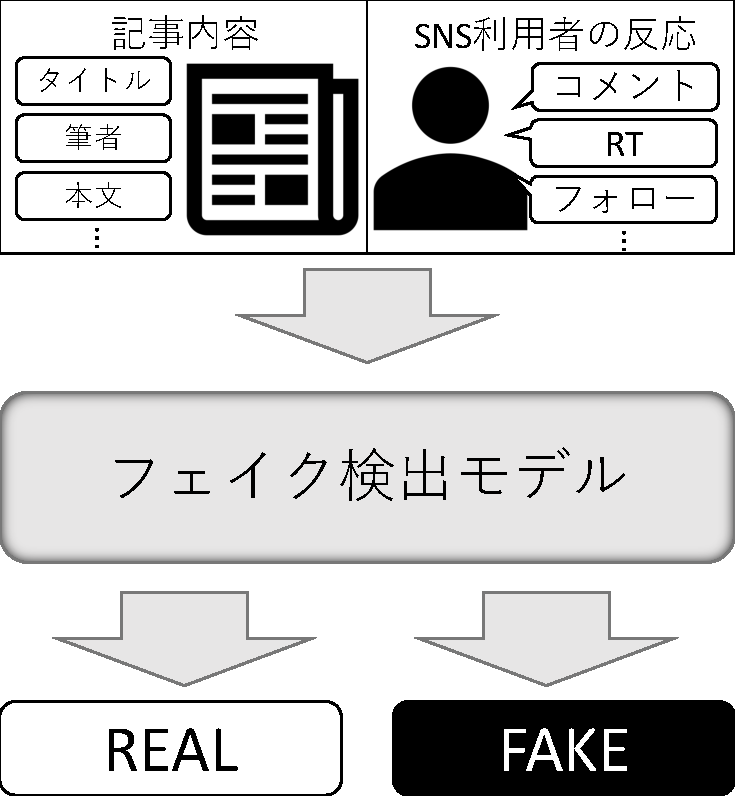
\includegraphics[width=0.3\textwidth]{figs/base_model.pdf}
    \vspace{-1cm} 
    \caption{フェイクニュース自動検出の基本的な流れ}
    \label{fig:objects}
\end{wrapfigure}
SNSの発展で情報を迅速かつ大量に取得・共有が容易になった一方、
悪意により他人を騙すために作られた\textbf{フェイクニュース}も拡散されやすくなった。
特に2020年からCOVID-19の影響による誤情報の拡散であるインフォデミックにより、
メタノール飲用による死亡事故\cite{iraninfo}といった事象が報告された。
以上から騙された人々により社会的損害が起きるため、
\underline{フェイクニュース拡散の早期抑制が必要である}\cite{snsinfo}。

フェイクニュース検出へ有識者が調査する\textbf{ファクトチェック}がある。
これは拡散ののち着手されるため、\underline{拡散抑制にはならない}。
そのため、自動でフェイクニュースを検出するべく深層学習によって
ファクトチェック結果をラベルとして、記事内容や利用者の反応から教師あり学習で自動検出する研究がある\cite{Wang:2018:EEA:3219819.3219903}。
%end 背景: 当該分野の状況 ====================

%begin 背景: 課題 ====================
\graysubsection{課題}
フェイクニュース自動検出が抱える課題は以下の通りである。

\begin{description}
    \vspace{-5mm}
    \setlength{\parskip}{0cm}
    \setlength{\itemsep}{0cm}
    \item[ニュースのタイムリー性] %\mbox{}\\
        ニュースという性質上、時間経過で扱われる情報が徐々に古くなりフェイクニュースの傾向変化への対応が難しくなる。
        先行研究によると学習・検証で入力するニュースの出来事を変えると検出性能が劣化する\cite{Wang:2018:EEA:3219819.3219903}。
        よって\underline{継続しデータセットを拡大する仕組みが必要}である。
    \item[SNSプラットフォームへの依存性] %\mbox{}\\
        SNS上で利用者からの反応を取得する場合、その形式は取得元のSNSプラットフォームに依存する。
        今後主流となるSNSが変わった場合、利用者層や時代の違いにより\underline{既存のデータでは対応できない}。
    \item[早期検出と正確性の両立] %\mbox{}\\
        記事内容に加えて利用者の反応(RT, コメント等)を扱うと検出性能が改善する\cite{Wu:2018:TFF:3159652.3159677}一方、
        利用者の反応を十分に得るには時間がかかり、\underline{高い正確性と早期検出を両立できない}。
    \item[日本語データセット不足] %\mbox{}\\
        深層学習による実現は、正解ラベルとして多量のファクトチェック結果を要する。
        このファクトチェックが活発な地域差の影響でデータセットが\textbf{英語に集中}\cite{fakenewsnet}している。
        もし\textbf{日本語を対象}とした場合、ラベル不足の影響により\underline{教師あり学習ができない}。
    \end{description}
%end 背景: 課題 ====================

%begin 着想に至った経緯 ====================
\graysubsection{本研究計画の着想に至った経緯}
私は修士課程で\underline{英文フェイクニュース早期検出の研究を行った}。
記事に対する利用者のコメントが検出に有用とする先行研究をベースに、
早期検出を想定して\underline{少ないコメントから更にコメント内容を自動生成}して検出するモデルを実装した。
実験にてコメントを生成した上で分類することでより多くのフェイクニュース検出を実現した(査読付き海外IEEE学会 発表済\cite{ines})。

一方、研究が進むつれて社会変化の激しさを実感した。
ニュースのトピックは日を追うごとに変化すると同時にフェイクニュースの内容も変わる上、
ユーザの反応が現れるSNSプラットフォームも近年は新しいサービスが提供されている。
この影響でこれまでの記事+SNS上の反応を扱う検出形式では、
データセット作成・モデル提供のみでは\underline{時代の変化に対応できない}。
よって\underline{記事を継続して収集する枠組み作り}に併せ、
ユーザの反応を\underline{SNSプラットフォームに左右されない形}で得る点の重要性に着目した。
%一方、国内研究会で発表したところ想定以上に日本語での実現に対する期待を受けた。
%日本は英語圏に比べファクトチェックされた記事が少なく、
%\underline{データセットを作ってモデルを実装するにはラベルが足りない}。
%このラベル不足を補う方法として、少量のラベル付き記事と多量のラベルなし記事に利用者の初期反応から
%弱いアノテーションを付加して学習を行う弱教師あり学習を行う研究\cite{mwss}に着目した。
%日本語で同じ構成のデータセットを作成し、分類を行うモデルを実装することで実現可能と考えた。

%end 着想に至った経緯 ====================

{\footnotesize 
%\vspace{1cm}
\begin{twobibliography}{99}
    \setlength{\parskip}{0cm}
    \setlength{\itemsep}{0cm}
    \bibitem{iraninfo} H. H-M, \textit{et al.} \textit{Critical Care} 24.1 2020: 1-3.
    \bibitem{snsinfo} S. Tasnim, \textit{et al.} \textit{JPMPH} 53.3 2020: 171-174.
    \bibitem{Wang:2018:EEA:3219819.3219903} Y. Wang, \textit{et al.} \textit{KDD'18}, pp. 849-857. 2018.
    \bibitem{Wu:2018:TFF:3159652.3159677} L. Wu \& H. Liu. \textit{WSDM '18},  pp. 637-645, 2018.
    \bibitem{fakenewsnet} K. Shu,\textit{et al.} \textit{Big Data 8.3} 2020: 171-188.
    \bibitem{coviddiff} Y. Bang, \textit{et al.} \textit{arXiv preprint arXiv:2101.03841} 2021.
    \bibitem{ines} Y. Yuta, \textit{et al.} \textit{INES}. 2020.
    \bibitem{mwss} K. Shu, \textit{et al.}  \textit{arXiv preprint arXiv:2004.01732} 2020.
\end{twobibliography}
}
% p01_background_01.tex
\KLEndSubject{F}



%#Split: 02_purpose_plan  
%#PieceName: p02_purpose_plan
% p02_purpose_plan_00.tex
\KLBeginSubjectWithHeaderCommands{02}{}{研究目的・内容等}{2}{F}{}{\DCPDFirstSubjectPageStyle}{\DCPDDefaultPageStyle}

\section{研究目的・内容等}
%    <<最大 2ページ>>

%s02_purpose_plan_dcpd
%begin 研究目的と研究計画short留意事項なし ====================
%begin 研究計画における研究目的、研究方法、研究内容 ====================
\graysubsection{①研究計画における研究目的、研究方法、研究内容}
\vspace{20pt}
\sbsbsection{研究目的}
本研究では、フェイクニュースの早期自動検出を日本語で実現するために、
データセットの作成から検出モデルの実装を目的とする。
さらに、汎化性能向上に向けてを目指す。

\sbsbsection{研究方法・研究内容}
以下の4つの目標を目指して研究を行う。
\begin{description}
    \item[目標Ⅰ] データセット作成に向けファクトチェック済記事とそうでない記事、同時にSNS上で記事に寄せられたコメントやユーザ情報等を収集する。
    \item[目標Ⅱ] 早期検出を想定した状況で高精度な真偽分類を行うモデルをユーザの初期反応から得られた弱いアノテーションと共に行う。
    \item[目標Ⅲ] 汎化性能向上に向けて内製以外のデータセットを用いても性能が劣化しないようモデルの改変を行う。
\end{description}

%end 研究計画における研究目的、研究方法、研究内容 ====================

%begin どのような計画で、何を、どこまで明らかにしようとするのか ====================
\graysubsection{②どのような計画で、何を、どこまで明らかにしようとするのか}
\vspace{20pt}
\sbsbsection{目標Ⅰ: 日本語の記事・真偽を含むデータセットを作成する(採用前 - 1年目)}
日本語での検出を実現するためには、まずはデータセットを作成する必要がある。
%完全教師あり学習・弱教師あり学習に問わず最低限必要なものは記事情報とファクトチェック結果による真偽ラベルである。
日本語ファクトチェック結果の取得には、特定非営利活動法人ファクトチェック・イニシアティブ(以下FIJ)が提供するFactCheck Naviを使用する。
2021年4月現在で600超件のファクトチェック結果が公表されている。%おり、FIJが提供するガイドライン\cite{fij}に基づき9種類のレーティングが行われている。
%今回はその中で``誤り''、``虚偽''、``ミスリード''、``不正確''、``根拠不明''と評価された記事をフェイクと扱う。
一方ファクトチェックにより正確と判断された事例はフェイクに比べて少な%く、2021年4月中旬現在FactCheck Naviの直近20件のファクトチェック結果は全てフェイクに該当する。
いため、正確なニュースとして大手新聞社やロイター通信等の記事を収集する。
また目標Ⅱに向けて正解ラベルがなく、弱いアノテーションを付加する対象である記事を追加する。
正確とみられるニュースは先述と同じく大手マスメディアが発信したニュースを扱い、
疑わしい記事としてFactCheck Naviによって虚偽と3回以上判断されたことがあるニュースサイトの他記事も収集対象とする。
最終的には真偽合わせて\bfundl{ラベル付き記事を約1200件}、\bfundl{ラベルなし記事を約5000件以上}収集を目指す。
ユーザの反応として、全記事を対象にSNS上で寄せられたコメントとしてTwitterにて記事URLを含むツイートも収集する。
\sbsbsection{目標Ⅱ: 弱教師あり学習によってラベル不足を補うモデルを構築する(1年目)}
ラベル付きユーザの反応を弱いアノテーションとして扱ってフェイクニュースを検出する方法は、
英文記事を対象にしたKai Shuらの研究で1例が示されている\cite{shu2020leveraging}。
ここではコメント群の感情値の標準偏差やコメント者の過去の投稿、そしてフォロー関係から弱いアノテーションを付加している。
これら3種の弱いアノテーションも併せて学習することで、推論時はユーザの反応を使わずに正確な早期検出を実現させている。
今回はこの3種類に加え、他に投稿者のプロフィールや使用された絵文字やハッシュタグといった情報で有用なものがないか模索する。

\sbsbsection{目標Ⅲ: トピックに左右されない汎化性能向上を模索する(2年目)}
更に提案手法の汎化性能を向上させるため、別のデータセットでも有用かどうか調べる。
日本語データセットは数が乏しいため、複数バリエーションがある英語で実験を行う予定である。
実験では学習と推論を同じデータセット内で完結させた時と別のデータセットで行った時を比較させ、
目標は2値(真・偽)分類時の総合指標であるF値の差が10パーセントポイント以下に留まることを目指す。

%end どのような計画で、何を、どこまで明らかにしようとするのか ====================

%begin 研究の特色・独創的な点 ====================
\graysubsection{③研究の特色・独創的な点}
\subsubsection*{本研究の特色}
日本語で自動検出を行う

早期検出を行う

変化する社会情勢に対しロバストである

\subsubsection*{先行研究との比較}
英語に偏重している

日本語データセットが不足している

\subsubsection*{予想されるインパクト・将来の見通し}
SNS利用者への注意喚起に活用可能

ファクトチェック支援システムへの活用

騙されて社会的損害や風評被害が発生するケースを未然に防ぐ

%end 研究の特色・独創的な点 ====================

%begin 申請者が担当する部分 ====================
\graysubsection{④申請者が担当する部分}
ぜんぶ
%end 申請者が担当する部分 ====================

%begin 受入研究機関と異なる研究機関での研究従事計画 ====================
\graysubsection{⑤受入研究機関と異なる研究機関での研究従事計画}
たりん
%end 受入研究機関と異なる研究機関での研究従事計画 ====================

\vspace{1cm}
{\footnotesize 
\begin{twobibliography}{99}
    \setlength{\parskip}{0cm}
    \setlength{\itemsep}{0cm}
    %\bibitem{fij} FIJ. 2019: ファクトチェック・ガイドライン
    \bibitem{shu2020leveraging} Kai S., \textit{et al.} ECML-PKDD 2020
\end{twobibliography}
}
%end 研究目的と研究計画short留意事項なし ====================
% p02_purpose_plan_01.tex
\KLEndSubject{F}



%#Split: 03_rights  
%#PieceName: p03_rights
% p03_rights_00.tex
\KLBeginSubjectWithHeaderCommands{03}{3}{人権の保護及び法令等の遵守への対応}{1}{F}{}{\DCPDFirstSubjectPageStyle}{\DCPDDefaultPageStyle}

\section{人権の保護及び法令等の遵守への対応}
%    <<最大 1ページ>>

% s09_rights
%begin 人権の保護及び法令等の遵守への対応 ====================
コメント取得を予定してしているSNSはTwitterである。
Twitter社は2020年3月より学術目的でTwitter APIの利用を自由化しているほか、
取得したツイートIDを含む情報をデータセットとして公開することも学術目的であれば認められている\cite{twitter_2020}。

また、先行研究が提供したデータセットを使用する場合は、提供者が示しているライセンスやポリシーを遵守する。

なお、学習済みモデルの公表は平成30年改正著作権法第30条4号により認められている。

%ただし、本研究では主観評価実験としてSNSユーザを対象としたアンケート調査を予定している。
%この調査により収集したデータは、個⼈の特定につながる情報を匿名化した上で解析を⾏い、
%解析結果の公表に際しては、匿名化を⾏ったデータを⽤い、個⼈情報の漏洩防⽌に配慮する。

\vspace{1cm}
{\footnotesize
	\begin{thebibliography}{99}
		\setcounter{enumiv}{11}
		\bibitem{twitter_2020} Twitter開発者ポリシーを分かりやすくアップデート, 2020年3月11日. (最終閲覧日 2020年4月19日) \url{https://blog.twitter.com/developer/ja_jp/topics/tools/2020/DevPolicyUpdate.html}
	\end{thebibliography}
}
%end 人権の保護及び法令等の遵守への対応 ====================

% p03_rights_01.tex
\KLEndSubject{F}



%#Split: 04_abilities  
%#PieceName: p04_abilities
% p04_abilities_00.tex
\KLBeginSubjectWithHeaderCommands{04}{4}{研究遂行力の自己分析}{2}{F}{}{\DCPDFirstSubjectPageStyle}{\DCPDDefaultPageStyle}

\section{研究遂行力の自己分析}
%    <<最大 2ページ>>

% s14_abilities
%begin 自己分析 ====================
%\DCPDInstructionsA\\% <-- 留意事項:これは消すか、コメントアウトしてください。
\noindent
\graybf{(1) 研究に関する自身の強み}

\sbsbsection{主体性}
私は高校3年次にバイオインフォマティクス(生命情報学)分野の研究活動として初めてプログラミングを行いWebクローラーを開発した(成果4)。
その後大学でコンピュータサイエンスの経験を積む中で、
%熊本地震や米国大統領選挙でフェイクニュース問題が多く取り沙汰されるようになった。
%誤った情報が広まって風評被害が出る事例は古今東西起きているものの、
%ことSNSが普及した現代社会では共有によって拡散のスピードが速く広くなる点に危機感を抱いた。
社会情勢の変化から自動で誤った情報を検出できないか考えるようになった。
学部〜修士課程でこの問題意識からフェイクニュース自動検出をテーマに据え、
指導教員を始め多くの研究者から助言を受けつつ\underline{主体的に研究を進めてきた}。
英文記事が対象のため、
\underline{積極的に海外学会を中心に成果を発表し}、\underline{研究内容や今後の発展について議論}を交わした。
\underline{既に1回査読付き海外IEEE学会で口頭発表}し(成果1)、
\underline{国内研究会でも2回口頭発表}を行った(成果2, 3)。

\sbsbsection{状況把握能力}
私が学部〜修士で行ってきた研究(成果1〜3)は、
特に海外で盛んに行われている研究である。
このため積極的に英語論文の調査を行い、
その研究内容を研究室内部のみならずときに他大学の学生へ共有することで、
フェイクニュースの自動検出を行う研究における現在の状況を仔細に把握できるようになった。
実際に学部論文(内容は成果2に近い)で引用した文献26件のうち24件が英語論文や記事であり、
修士論文(内容は成果3に近い)で引用した文献76件のうち74件が英語論文や記事であった。
このように私は\underline{貪欲な海外論文調査に裏打ちされた状況把握能力}があると考える。

\sbsbsection{実装能力}
私は\underline{産学問わず}プログラミング活動を行ってきた。
最初のプログラミング開発(成果1)では、実装に適した言語の選定から、独習〜実装、
そしてポスター作成まで一貫して大学合格発表直後から発表会までの2週間で独力で行った。
このプログラミング能力は大学入学直後も発揮し続け、
産業界ではこれまで2社で3ヶ月以上継続したエンジニア活動を行っている(成果6, 7)ほか、
1〜2ヶ月に及ぶ短期エンジニアインターンシップも2社で行った(成果8, 9)。
一方学部研究(成果2)では3カテゴリ分類モデルの実装を独力で行った。
また修士研究(成果1, 3)では、
既存のフェイクニュース生成モデルGrover\cite{grover}のソースコードを改変する形で記事ではなくコメントを生成するシステムを構築した。
よって私には豊富な開発経験がもたらす実装能力があると確信する。

\sbsbsection{プレゼン・コミュニケーション能力}
\underline{研究会に限らずリモート開催された海外学会にも積極的に参加}し、
研究者達とのコミュニケーションを積極的に行った。
また他大学との合同ゼミにも参加し、別分野の研究に対する理解を深めている。

私は大学入りしてから小中高校生を対象としたプログラミング教室の立ち上げから関与を続け、
講師としても2年半かけて活動を続けた(成果5)。
具体的には教える言語(Python)の習得を目的とした輪講に参加し、
講師として開講から2年間にわたり毎週受講生の学習のメンタリングを行った。
受講生が分からないと申告した部分は実際にその部分が不明なのか、それとも前提とする部分から既に不明なのか、
丁寧な聞き込みから特定を行い指導することで自学自習が進みやすくなるよう意識し、
また受講生が自主制作したいプログラムが現在の技量に対して高度過ぎる場合は、
段階となりそうな例を示して開発するよう指導した。
こういった経験で、\underline{他者の視点に立った説明が必要だと強く認識}した。

以上から\underline{相手が小学生でも物事を分かりやすく伝えられるプレゼン能力}があると考える。
%\DCPDInstructionsB% <-- 留意事項:これは消すか、コメントアウトしてください。

\sbsbsection{成果: 国際会議における発表}
(以下1件 査読あり・論文及び口頭発表)
\vspace{-4mm}
\begin{enumerate}
    \setlength{\parskip}{0cm}
    \setlength{\itemsep}{0cm}
    \item \underline{$\circ$ Yuta Yanagi}, Ryouhei Orihara, Yuichi Sei, Yasuyuki Tahara, and Akihiko Ohsuga.\\
    ``Fake news detection with generated comments for news articles''.\\
    The 24th IEEE International Conference on Intelligent Engineering Systems 2020,\\
    (Reykjavík, Iceland) Virtual event due to COVID-19, July 2020.
\end{enumerate}

\sbsbsection{成果: 国内学会やシンポジウムにおける発表}
(以下2件 査読なし・口頭発表)
\vspace{-3mm}
\begin{enumerate}
    \setcounter{enumi}{1}
    \setlength{\parskip}{0cm}
    \setlength{\itemsep}{0cm}
    \item \underline{$\circ$ 栁裕太}、田原康之、大須賀昭彦、清雄一\\
        「画像付きフェイクニュースとジョークニュースの検出・分類に向けた機械学習モデルの検討」、\\
        日本ソフトウェア科学会 2018年度 MACC研究発表会、
        大分、2019年3月
    \item \underline{$\circ$ 栁裕太}、折原良平、清雄一、田原康之、大須賀昭彦\\
        「フェイクニュースの早期自動検出に向けたニュース記事コメント生成モデルの提案」、\\
        言語理解とコミュニケーション研究会(NLC) 第17回テキストアナリティクス・シンポジウム、\\
        オンライン、2021年2月
\end{enumerate}
(以下1件 査読なし・ポスター発表)
\vspace{-4mm}
\begin{enumerate}
    \setcounter{enumi}{3}
    \setlength{\parskip}{0cm}
    \setlength{\itemsep}{0cm}
    \item \underline{$\circ$ 栁裕太}、葛西透麿、 森谷薫平、神谷岳洋、藤原徹、木村健太、榎本裕介\\
        「CaD428の変異遺伝子の機能解析ツールの汎用化」、\\
        広尾学園高校医進・サイエンスコース研究成果報告会、
        東京、2015年3月
\end{enumerate}

\sbsbsection{成果: 学外活動歴}
\begin{enumerate}
    \setcounter{enumi}{4}
    \setlength{\parskip}{0cm}
    \setlength{\itemsep}{0cm}
    \item UECプログラミング教室講師、2016年5月〜2018年3月
    \item アメリエフ株式会社におけるエンジニア活動、2016年8月〜2018年3月
    \item 株式会社justInCase Technologiesにおけるエンジニア活動、2018年10月〜活動中
    \item 株式会社フィックスターズにおける短期エンジニアインターンシップ活動、2019年7〜8月
    \item 株式会社アカツキにおける短期バックエンドエンジニアインターンシップ活動、2020年7月
\end{enumerate}

\vspace{5mm}
\noindent
\graybf{(2) 今後研究者として更なる発展のため必要と考えている要素}
\sbsbsection{要素Ⅰ: 学術的成果と社会問題の最前線の間にあるギャップを埋めるための発想力}
フェイクニュースの自動検出を行う研究は世界的に広く行われており、
それぞれが独自の発想を追加している。
この付加する独自の発想は、ときに他分野から得た知見がもたらす。
よって技術面では自然言語処理に限らず、利用者の拡散を考慮するためのグラフネットワークや、
既知の情報を利用するためのナレッジグラフ技術など、
\underline{幅広い分野の研究に論文を通して触れる}必要がある。
具体的にはフェイクニュースの自動検出に限らず、自然言語処理や画像処理、
そしてナレッジグラフなど、関連のありそうな分野全体に広げることで実現できると考えている。

\sbsbsection{要素Ⅱ: 多彩な分野や言語・地域圏の研究者らと活発な議論を交わす能力}
要素Ⅰの実現には、論文のみならず実際に議論を交わすことで更に深い理解を得ることが重要である。
また海外で研究が活発に行われていることから、知見のアップデートも頻繁に行うことも必要である。
よって\underline{分野・言語問わず多くの研究者達とプラットフォームを問わない深い議論が研究の発展をもたらす}と考える。

\sbsbsection{要素Ⅲ: 研究で得られた成果をどんな聞き手でも分かりやすく伝えられる表現力}
新型コロナウイルス感染症蔓延の影響もあり、発表の機会や形式が大きく制限されたまま修士研究を終えた。
オンライン形式での発表での経験を積めた一方、人前で発表する機会はあまり多くの経験を積められないままである。
それゆえ、\underline{場所を問わず誰が相手でも研究を分かりやすく伝える経験を積む}必要が例年以上に必要と考える。
%end 自己分析 ====================

%\vspace{1cm}
{\footnotesize
	\begin{thebibliography}{99}
		\setcounter{enumiv}{13}
		\bibitem{grover} R. Zellers, \textit{et al. NeurIPS 2019}
        \bibitem{uecprog} 安部博文, 【第1期子供のためのプログラミング教室(4)記録】, 国立大学法人電気通信大学インキュベーション施設, 2016年5月29日(最終閲覧日 2021年5月3日) \url{http://www.uecincu.com/programming/programming_160529.html}
        \bibitem{amelieff} アメリエフ株式会社「4月21日(金)「医療ビッグデータを活用して世界を変える! 学生インターンMeetup 2017春」開催のお知らせ」, 2017年4月7日(最終閲覧日 2021年5月3日) \url{https://amelieff.jp/170407/}
        \bibitem{jic-tech} 「株式会社 justInCaseTechnologies | 保険を変える保険テック会社」, 2020年12月1日(最終閲覧日 2021年5月3日) \url{https://justincase-tech.com/}
	\end{thebibliography}
}
% p04_abilities_01.tex
\KLEndSubject{F}



%#Split: 05_my_ambitions  
%#PieceName: p05_my_ambitions
% p05_my_ambitions_00.tex
\KLBeginSubjectWithHeaderCommands{05}{5}{目指す研究者像等}{1}{F}{}{\DCPDFirstSubjectPageStyle}{\DCPDDefaultPageStyle}

\section{目指す研究者像等}
%    <<最大 1ページ>>
\begin{spacing}{1.08}
% s17_my_ambitions
\noindent
\graybf{(1)目指す研究者像} {\footnotesize ※目指す研究者像に向けて身に付けるべき資質も含め記入してください。}

%begin 目指す研究者像 ====================
私は幼少期からコンピュータに触れる機会が多かった影響で、コンピュータサイエンスやプログラミングに興味を持った。
その後広尾学園高校で初めてプログラミングを含む研究活動を通し、自分で問題解決へ調査から発表まで行う楽しさを知った。
この2つの経験から、\underline{興味のある分野を研ぎ究める}と同時に\underline{社会問題を解決して人々の生活を幸せ}にしたいと考えるようになった。

大学入学から研究活動を開始するまでの間、
熊本地震や米国大統領選挙でフェイクニュース問題が頻繁に取り沙汰された。
誤った情報が広まることで騙された人々によって多くの社会的損害が発生しており、
中には故意に作られたものも含まれていた。
あまりに速く拡散されるある種``広め得''な状況を、私はフェアではないと感じるようになった。
誤った情報が広まって風評被害が出る事例は古今東西起きているものの、
ことSNSが普及した現代社会では共有によって拡散のスピードが速く広くなる点に危機感を抱いた。
事実と異なる情報が訂正が入る前に広く拡散され、
\underline{騙されて誤った風評が残り不幸になる人を0にしたい}という考えがテーマ選定の大きな動機である。

修士研究を終えるまでの3年もの間、このテーマで研究を進めていくなかでフェイクニュースを自動で検出し利用者の拡散を抑制する難しさを認識した。
フェイクニュースは読者を騙すため精巧なものも多く、
真偽ラベルを付加するアノテーションを専門家以外に任せにくい上に、
判断結果をただ見せるだけでは読者を納得させる説得力を持たせにくい。
これらに対処するため、先行研究ではその解決に向けて自然言語処理に限らず幅広い分野の知見を取り入れている。
多くのアプローチが試されている中で、
大きな新規性をもたらすための\underline{新たな発想をいかに取り入れるかが重要}である点を修士研究までの3年間で痛感した。
その実現に向けて、他分野にも広く精通するためには\underline{国内外の研究者達と活発な議論を通して理解を深める}必要性も認識している。

また自動検出を利用者によるフェイクニュース拡散の抑止に繋げるためには、
利用者に納得できる形で提供する重要性も同時に認識している。
判断結果に説得力がないと、利用者による信頼を得られず拡散抑止への効果が薄れるためである。
研究そのものも同じく、社会に対してわかりやすい説明を行うことで更に提供モデルの効果も強くなる。
このように\underline{自己完結のみならず成果を他人に伝えるまでが研究}と考える。

最終的にはフェイクニュースの自動検出を発展させ、
ニュースやSNS上での拡散現象から利用者による拡散活動を解き明かし、
\underline{誤った情報で被害を受ける人を0にする}ことを目指す。
さらに今後はアカデミックポストとしてアウトリーチ活動も積極的に行うことで、
研究と同時に後輩学生・研究者・SNS利用者へ\underline{分かりやすい説明を通して持続可能な社会の発展へ成果を還元できる研究者}を目指す。

%end 目指す研究者像 ====================

\vspace{5mm}
\noindent
\graybf{(2)上記の「目指す研究者像」に向けて、特別研究員の採用期間中に行う研究活動の位置づけ}

%begin 研究活動の位置づけ ====================
特別研究員の採用期間中に行う研究活動のなか、
4-(2)で挙げた今後研究者としてさらなる発展のため必要と考えている要素の習得を通して、
\underline{学術研究で得た知見を直接SNS利用者を含む日本社会に還元}する研究者を目指す。

その実現に向け、査読付き国際会議ないしは国際論文誌への論文発表をはじめ、
国内・国際会議での口頭発表も積極的に行う。
また、自然言語処理コミュニティに限らず国内ニュースメディアと積極的に連携を行い、
フェイクニュースの自動検出に関連した共同研究の実現が理想である。

特別研究員として研鑽を重ねていき、
現状の研究への新たな発想を追加し、実現に向けて幅広い人々と議論を重ね、得られた成果を端的に説明することが、
\underline{能動的に一貫して社会課題を解決へ自ら導く研究者}として大成へと導く。
その実現の大きな足がかりが本研究計画である。
%end 研究活動の位置づけ ====================
\end{spacing}
% p05_my_ambitions_01.tex
\KLEndSubject{F}



%#Split: 99_tail
% hook9 : right before \end{document} ============
 % pieces
\end{document}

